\clearpage
\section{Practice Problems}
Let's do some practice problems, shall we? I'll only give a couple, each increasing in difficulty.

\begin{problem}
    Let the function $f$ be $f(x) = x^2$. Translate (move) this function $2$ units to the right and $1$ unit down. Write your answer as a new function $g$.
\end{problem}
\begin{solution}
    We're given two translations: A horizontal translation $h$ and a vertical translation $k$. We're asked to move this function two units to the right, meaning $h = 2$. We're then asked to move this function $1$ unit down, meaning $k = -1$. Apply these to the template $g(x) = f(x - h) + k$.
    Plugging these into the function yields the answer $\boxed{g(x) = (x - 2)^2 - 1}$.
\begin{center}
    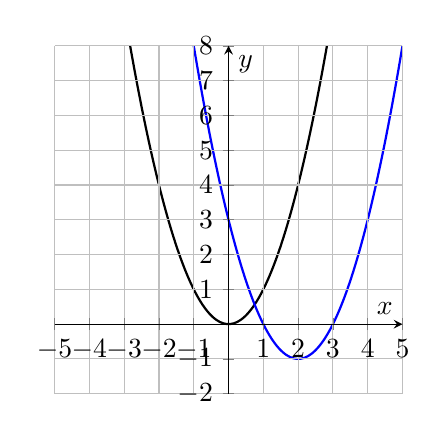
\begin{tikzpicture}
        \begin{axis} [
            axis lines=middle,
            xlabel = $x$, ylabel = {$y$},
            xmin = -5, xmax = 5,
            ymin = -2, ymax = 8,
            xtick distance={1}, ytick distance={1},
            grid = both,
            width = 6cm,
            height = 6cm,
            smooth,
            axis on top
        ]

            \addplot[black, thick, smooth, domain = -5:5, samples = 100]{x^2};
            \addplot[blue, thick, smooth, domain = -5:5, samples = 100]{(x - 2)^2 - 1};
        \end{axis}
    \end{tikzpicture}\\
    $f(x) = x^2$ (Black), 
    $g(x) = (x - 2)^2 - 1$ (Blue),
\end{center}
\end{solution}\clearpage
\begin{problem}
    Let the function $f$ be $f(x) = \sqrt{x}$. Apply a vertial stretch with a factor of $3$ and horizontal stretch with a factor of $\frac{1}{2}$. Write your answer as a new function $g$.
\end{problem}
\begin{solution}
We're given two transformations: A vertial stretch $a$ and a horizontal stretch $b$. We're asked to vertically stretch this function by a factor of $3$, meaning $a = 3$, and horizontally stretch this function by a factor of $\frac{1}{2}$, meaning $b = \frac{1}{2}$. Apply these to the template $g(x) = af\left(\dfrac{1}{b}x \right)$. 

The vertical stretch is easy, just slap the $3$ in for $a$. The horizontal stretch, on the other hand, is more tricky. We know that $b = \dfrac{1}{2}$, but plugging that in gives $\dfrac{1}{1/2}$. This is a complex fraction and serves only to complicate things. To get rid of this, we multiply the numerator and denominator by the reciporical of the denominator.
\[
    \frac{1}{\frac{1}{2}}\cdot \frac{\frac{2}{1}}{\frac{2}{1}} =
    1 \cdot \frac{2}{1} = 1 \cdot 2 = 2
\]
Thus, our final answer is $\boxed{g(x) = 3\sqrt{2x}}$.
\begin{center}
    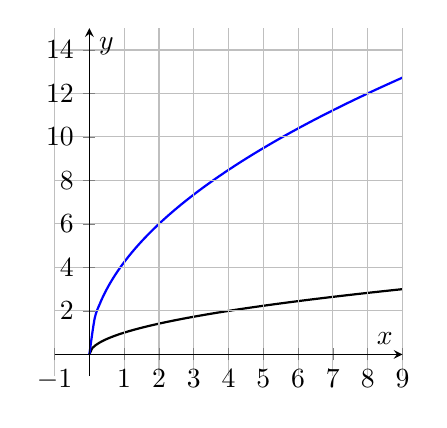
\begin{tikzpicture}
        \begin{axis} [
            axis lines=middle,
            xlabel = $x$, ylabel = {$y$},
            xmin = -1, xmax = 9,
            ymin = -1, ymax = 15,
            xtick distance={1}, ytick distance={2},
            grid = both,
            width = 6cm,
            height = 6cm,
            smooth,
            axis on top
        ]

            \addplot[black, thick, smooth, domain = 0:9, samples = 100]{sqrt(x)};
            \addplot[blue, thick, smooth, domain = 0:15, samples = 100]{3 * sqrt(2 *x)};
        \end{axis}
    \end{tikzpicture}\\
    $f(x) = x^2$ (Black), 
    $g(x) = (x - 2)^2 - 1$ (Blue),
\end{center}
\end{solution} \clearpage
\begin{problem}
    Let the function $f$ be $f(x) = \dfrac{1}{x}$. Translate the function $3$ units to the left and $5$ units up. Transform the function with a vectical stretch factor of $2$ and horizontal stretch factor of $3$. Reflect the function over the $y$-axis. Write your answer as a new function $g$.
\end{problem}
\begin{solution}
    There are a lot of things we need to do to this function, so let's list them one at a time.
    \begin{itemize}
        \item Move $3$ units left ($h = 3$).
        \item Move $5$ units up ($k = 5$).
        \item Vertically stretch by a factor of $2$ ($a = 2$).
        \item Horizontally stretch by a factor of $3$ ($b = 3$).
        \item Reflect over the $y$-axis (We'll worry about this later).
    \end{itemize}
    With what we've gathered so far, we can create a template:
    \begin{align*}
        g(x) &= 2f\left(\frac{1}{3}(x - 3) \right) + 5 \\
        \intertext{From here, we can plug everything in}
        g(x) &= 2\left(\frac{1}{\frac{1}{3}(x - 3)} \right) + 5
    \end{align*}
    Now we can reflect over the $y$-axis. Remember that the $y$-axis is the line $x = 0$. It's the vertical line that goes straight through the $xy$-plane. Since we're reflecting from left to right, we must multiply $b$ by $-1$. This gives
    \[
        g(x) = 2\left(\frac{1}{-\frac{1}{3}(x - 3)} \right) + 5 \text{.}
    \]
    Now, we begin solving:
    \begin{align*}
    g(x) &= \frac{2}{-\frac{1}{3}(x - 3)}\left(\frac{\frac{3}{1}}{\frac{3}{1}} \right) + 5 \\
    &= \frac{6}{-(x - 3)} + 5 \\
    &= 5 - \frac{6}{x - 3}
    \end{align*}
\begin{center}
    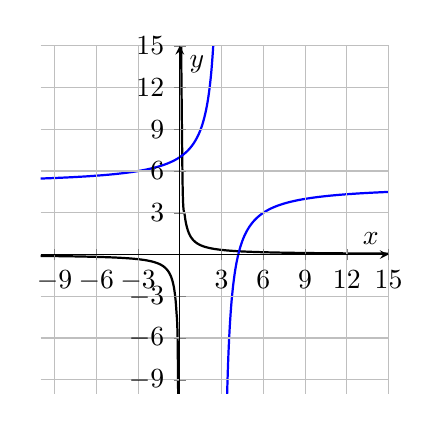
\begin{tikzpicture}
        \begin{axis} [
            axis lines=middle,
            xlabel = $x$, ylabel = {$y$},
            xmin = -10, xmax = 15,
            ymin = -10, ymax = 15,
            xtick distance={3}, ytick distance={3},
            grid = both,
            width = 6cm,
            height = 6cm,
            smooth,
            axis on top
        ]

            \addplot[black, thick, smooth, domain = -10:-0.05, samples = 100]{1 / x};
            \addplot[black, thick, smooth, domain = 0.05:15, samples = 100]{1 / x};
            \addplot[blue, thick, smooth, domain = -10:2.8, samples = 100]{5 - (6 / (x - 3))};
            \addplot[blue, thick, smooth, domain = 3.1:15, samples = 100]{5 - (6 / (x - 3))};
        \end{axis}
    \end{tikzpicture}\\
    $f(x) = \frac{1}{x}$ (Black), 
    $g(x) = 5 - \frac{6}{x - 3}$ (Blue),
\end{center}
Note that you could also write this function as
\[
    g(x) = \frac{6}{3 - x} + 5 \text{.}
\]
and get the same result. That's how I'd write it. You could also just leave it as
\[
    g(x) = \frac{6}{-(x - 3)} + 5 \Longrightarrow \boxed{g(x) = -\frac{6}{x - 3} + 5} \text{.}
\]
It's all stylistic/presentation preferences.
\end{solution}